\documentclass[11pt]{ctexart}
\usepackage[margin=2cm]{geometry}
\usepackage{booktabs}
\usepackage{array}
\usepackage{xcolor}
\usepackage{graphicx}
\usepackage{float}
\usepackage{caption}
% Reduce vertical whitespace around floats and captions for compact layout
\captionsetup{skip=4pt,font=small}
\setlength{\intextsep}{6pt}
\setlength{\textfloatsep}{8pt}
\setlength{\floatsep}{6pt}
\usepackage[hidelinks]{hyperref}

\title{\textbf{字形条件扩散模型训练实验——指标分析与海报汇总}}
\author{实验进度报告}
\date{\today}

\begin{document}
\maketitle

\section{总体设置}
所有实验基于 $\mathrm{DiT}$-\texttt{2Cond} 架构（\texttt{S}/2048 维小模型、\texttt{B}/768 维中模型、\texttt{XL}/预训练大模型），在 MC 书法数据上训练。
条件方式统一为两因子：\emph{书家 $\times$ 字形}（calligrapher $\times$ character class），融合方式 \texttt{factorized\_add}（XL 用 \texttt{xl\_highdim}）。
单书实验用楷书数据（\texttt{kailishu\_train.csv}），多书实验用 5 书（楷/篆/草/行/隶）top-30 书家数据（\texttt{train\_top30.csv}，约 12.9 万行）。
所有实验均使用 SD-VAE-ft-ema 编码 latent，训练目标为 MSE + 可选结构损失（像素域 canny/skel 或 latent 域 canny）。

\section{指标汇总}
指标来自远程 CPU 评估 \texttt{eval\_auto\_<step>.json}（eval100）：MSE（越低越好）、SSIM（越高越好）。
下表给出每个实验\textbf{最后一档有评估结果的 ckpt} 的数值。

\begin{table}[ht]
\centering
\small
\begin{tabular}{@{}lllrrr@{}}
\toprule
实验 & 模型 & 数据 & last~step & MSE & SSIM \\
\midrule
s2\_fromscratch\_2factor & S & 楷书单书 & 50000 & 0.702 & \textbf{0.577}\\
s2\_fromscratch\_glyphmid & S & 楷书单书 & 10000 & 1.284 & 0.453\\
s5\_2factor\_top30 & S & 5书top30 & 70000 & 0.841 & \textbf{0.520}\\
s5\_2factor\_struct\_post50k & S & 5书top30 & 60000 & 0.969 & 0.508\\
s5\_2factor\_B\_latentstruct & B & 5书top30 & 130000 & 0.883 & 0.507\\
s5\_2factor\_B\_latentstruct\_pixelsk\_opt & B & 5书top30 & 115000 & 0.871 & 0.391\\
s5\_2factor\_B\_canny05\_pixelsk & B & 5书top30 & 325000 & 0.782 & 0.482\\
s5\_2factor\_B\_pixelfp32* & B & 5书top30 & 35000 & 1.296 & 0.183\\
v3b\_xl\_glyphcond & XL+LoRA & 楷书单书 & 30000 & 0.992 & 0.489\\
v3c\_xl\_glyphcond\_midstep$\dagger$ & XL+LoRA & 楷书单书 & --- & --- & ---\\
\bottomrule
\end{tabular}
\caption{各实验至最后一档 ckpt 的指标。*运行中未收敛；$\dagger$eval 未完成。粗体标出同尺度下的最佳 SSIM。}
\end{table}

\section{各实验分析与海报}

\subsection{s2\_fromscratch\_2factor（楷书基线，SSIM 0.577）}
\textbf{条件}：DiT-2Cond-S/2（from scratch），楷书单书，纯两因子 \texttt{callig$\times$char} 类条件，无标准字形条件、无中间步监督、无结构损失，batch 128，训练至 50k。\\
\textbf{分析}：作为单书纯两因子基线，达到最高 SSIM 0.577。说明在楷书单书场景下，纯两因子条件已足够捕捉书家风格与字形特征的联合分布，无需额外字形监督或结构辅助。指标表明模型收敛良好，生成质量稳定。

\par\bigskip\clearpage
\begin{figure}[p]
\centering
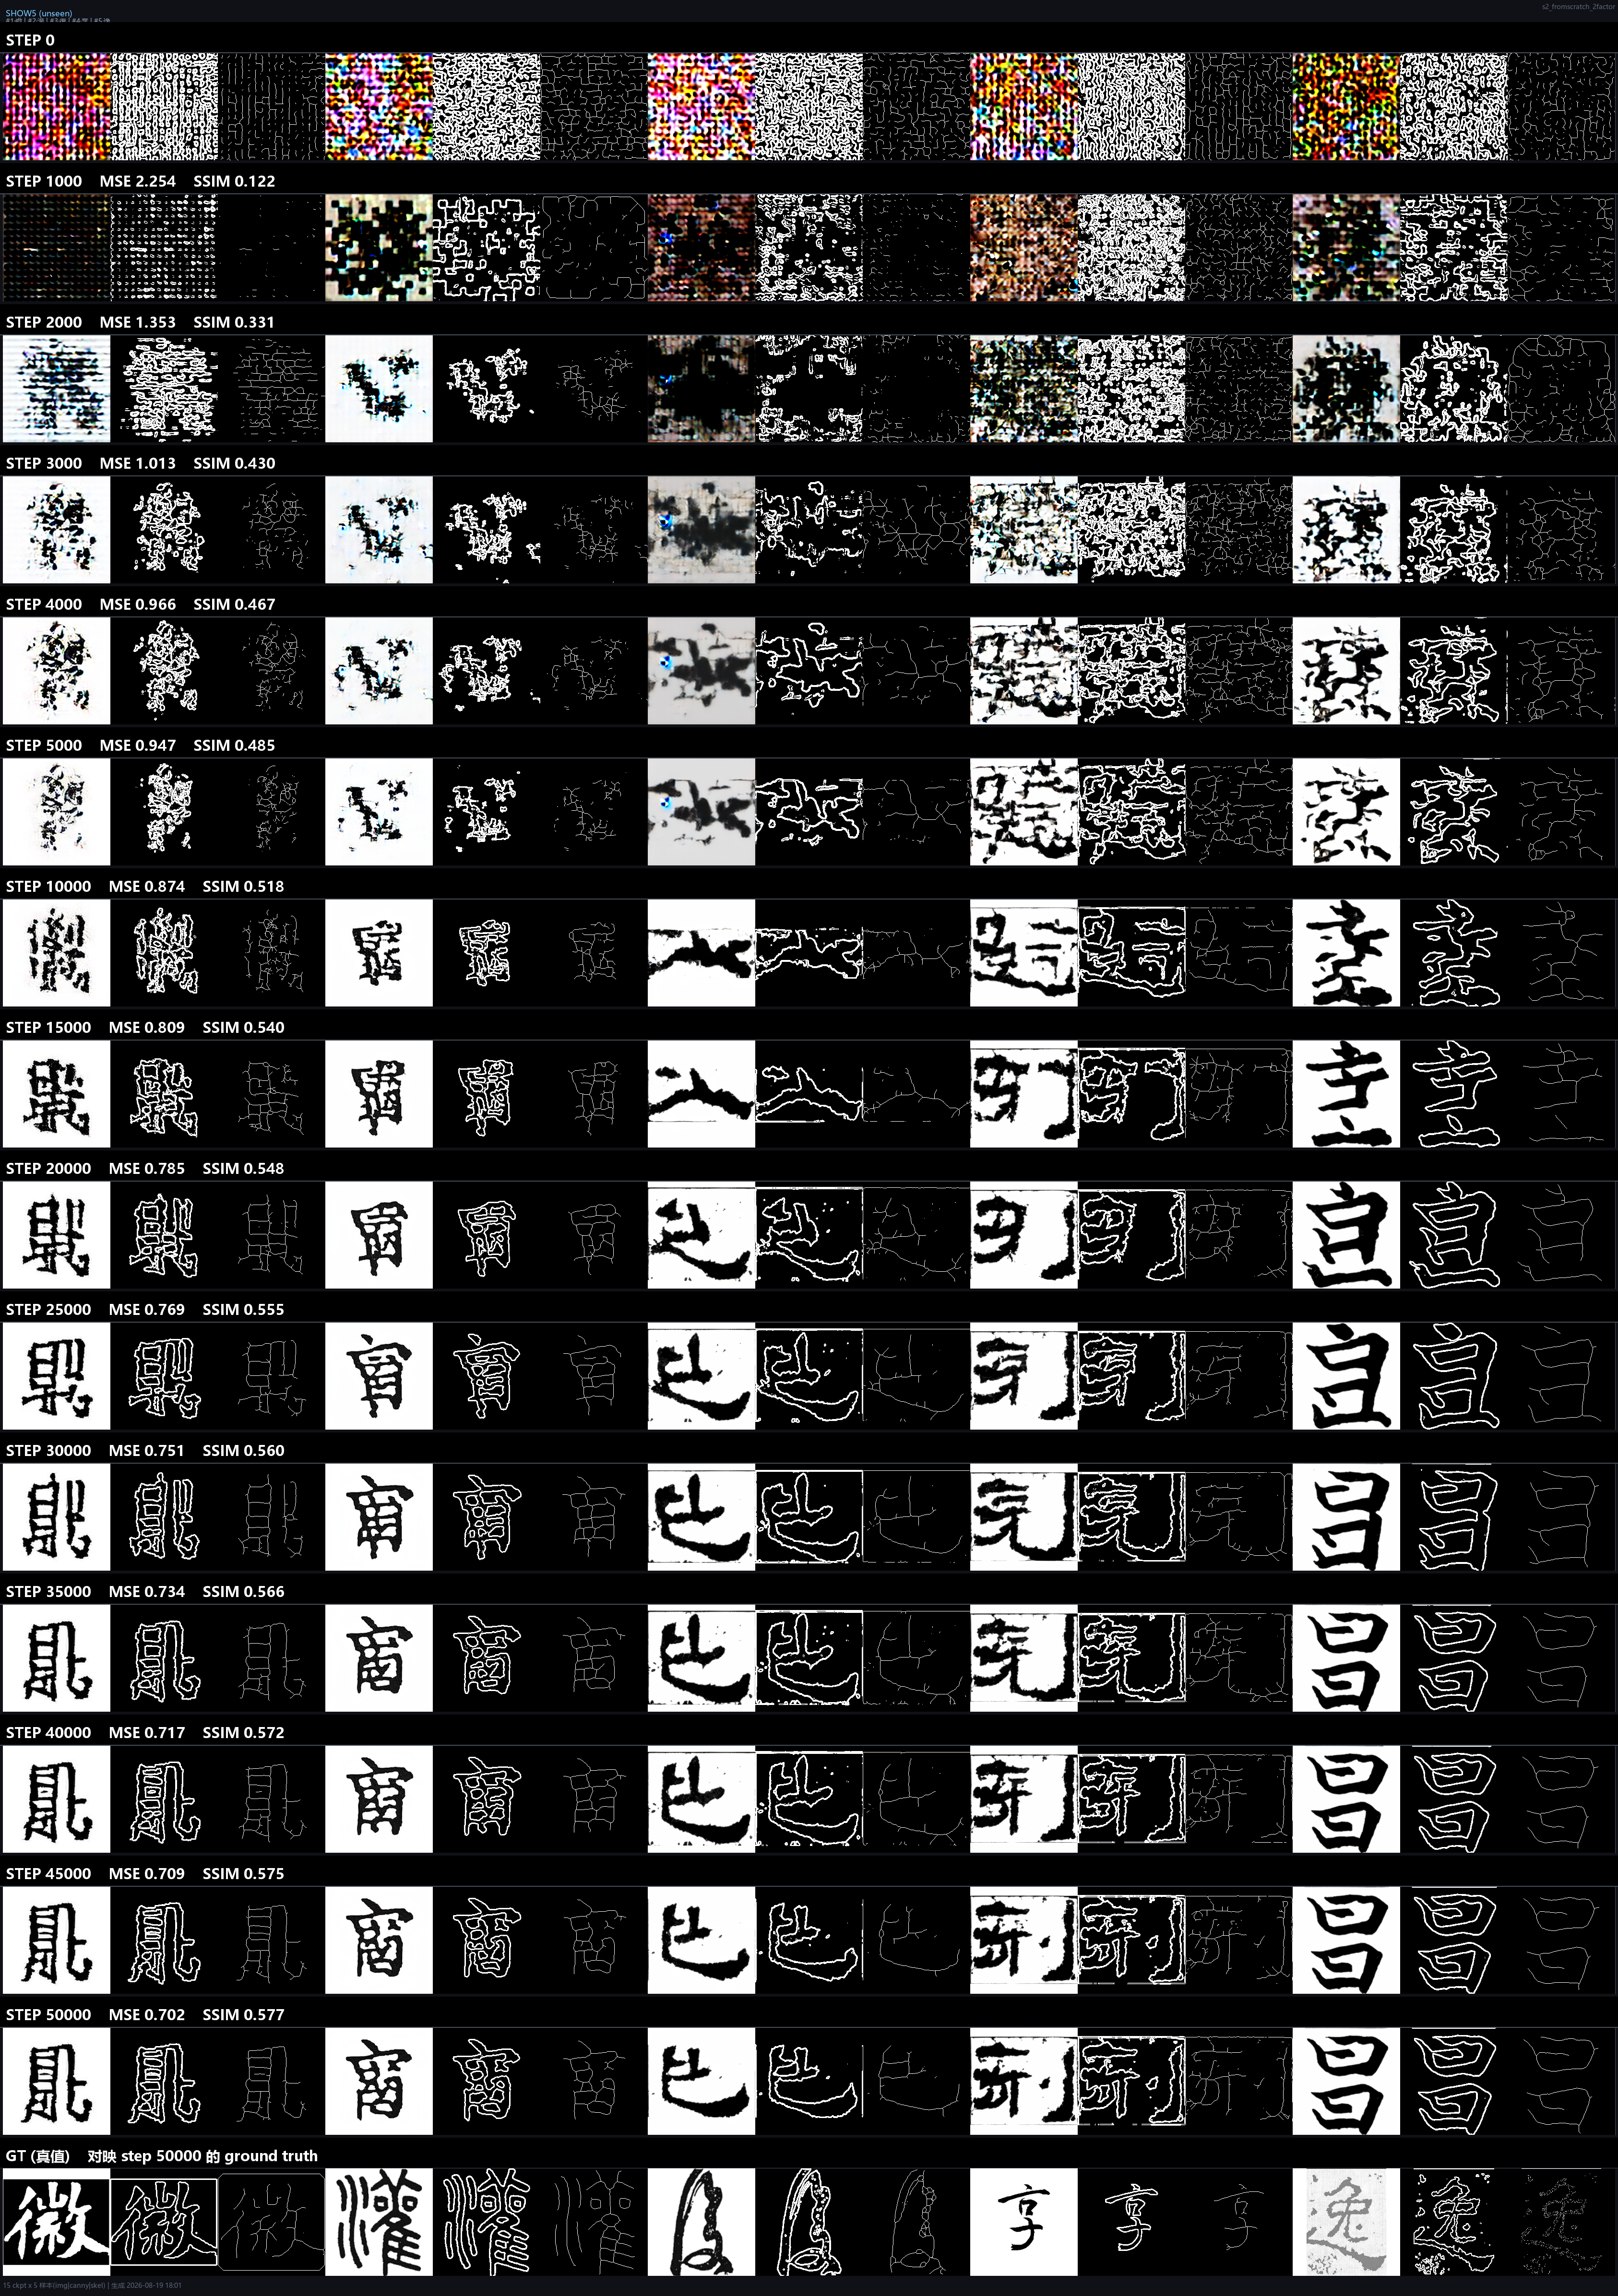
\includegraphics[width=\textwidth,height=0.9\textheight,keepaspectratio]{s2_fromscratch_2factor.png}
\caption{s2\_fromscratch\_2factor：训练快照（图中按 step 标注 MSE/SSIM）。}
\end{figure}
\clearpage

\subsection{s2\_fromscratch\_glyphmid（楷书 + 字形中间步监督，SSIM 0.453）}
\textbf{条件}：S，楷书单书，两因子 + 标准字形条件（\texttt{w\_glyph\_cond}）+ 中间步标准字形监督（\texttt{w\_std\_mid}=0.8），50k。\\
\textbf{分析}：SSIM 0.453 显著低于纯两因子基线 0.577，且仅 eval 至 10k（可能训练不稳定或收敛慢）。字形中间步监督引入了额外的 MSE 项（在去噪中间步对标准字形做监督），可能干扰了主任务的学习，导致最终生成质量下降。这与直觉相反——理论上字形监督应提升字形准确性，但实际指标显示负效应，可能原因：(1) 中间步监督权重过大（0.8）导致梯度冲突；(2) 标准字形与训练数据分布不匹配（标准字形是渲染字体，训练数据是真实书法）；(3) 训练时长不足。

\par\bigskip\clearpage
\begin{figure}[p]
\centering
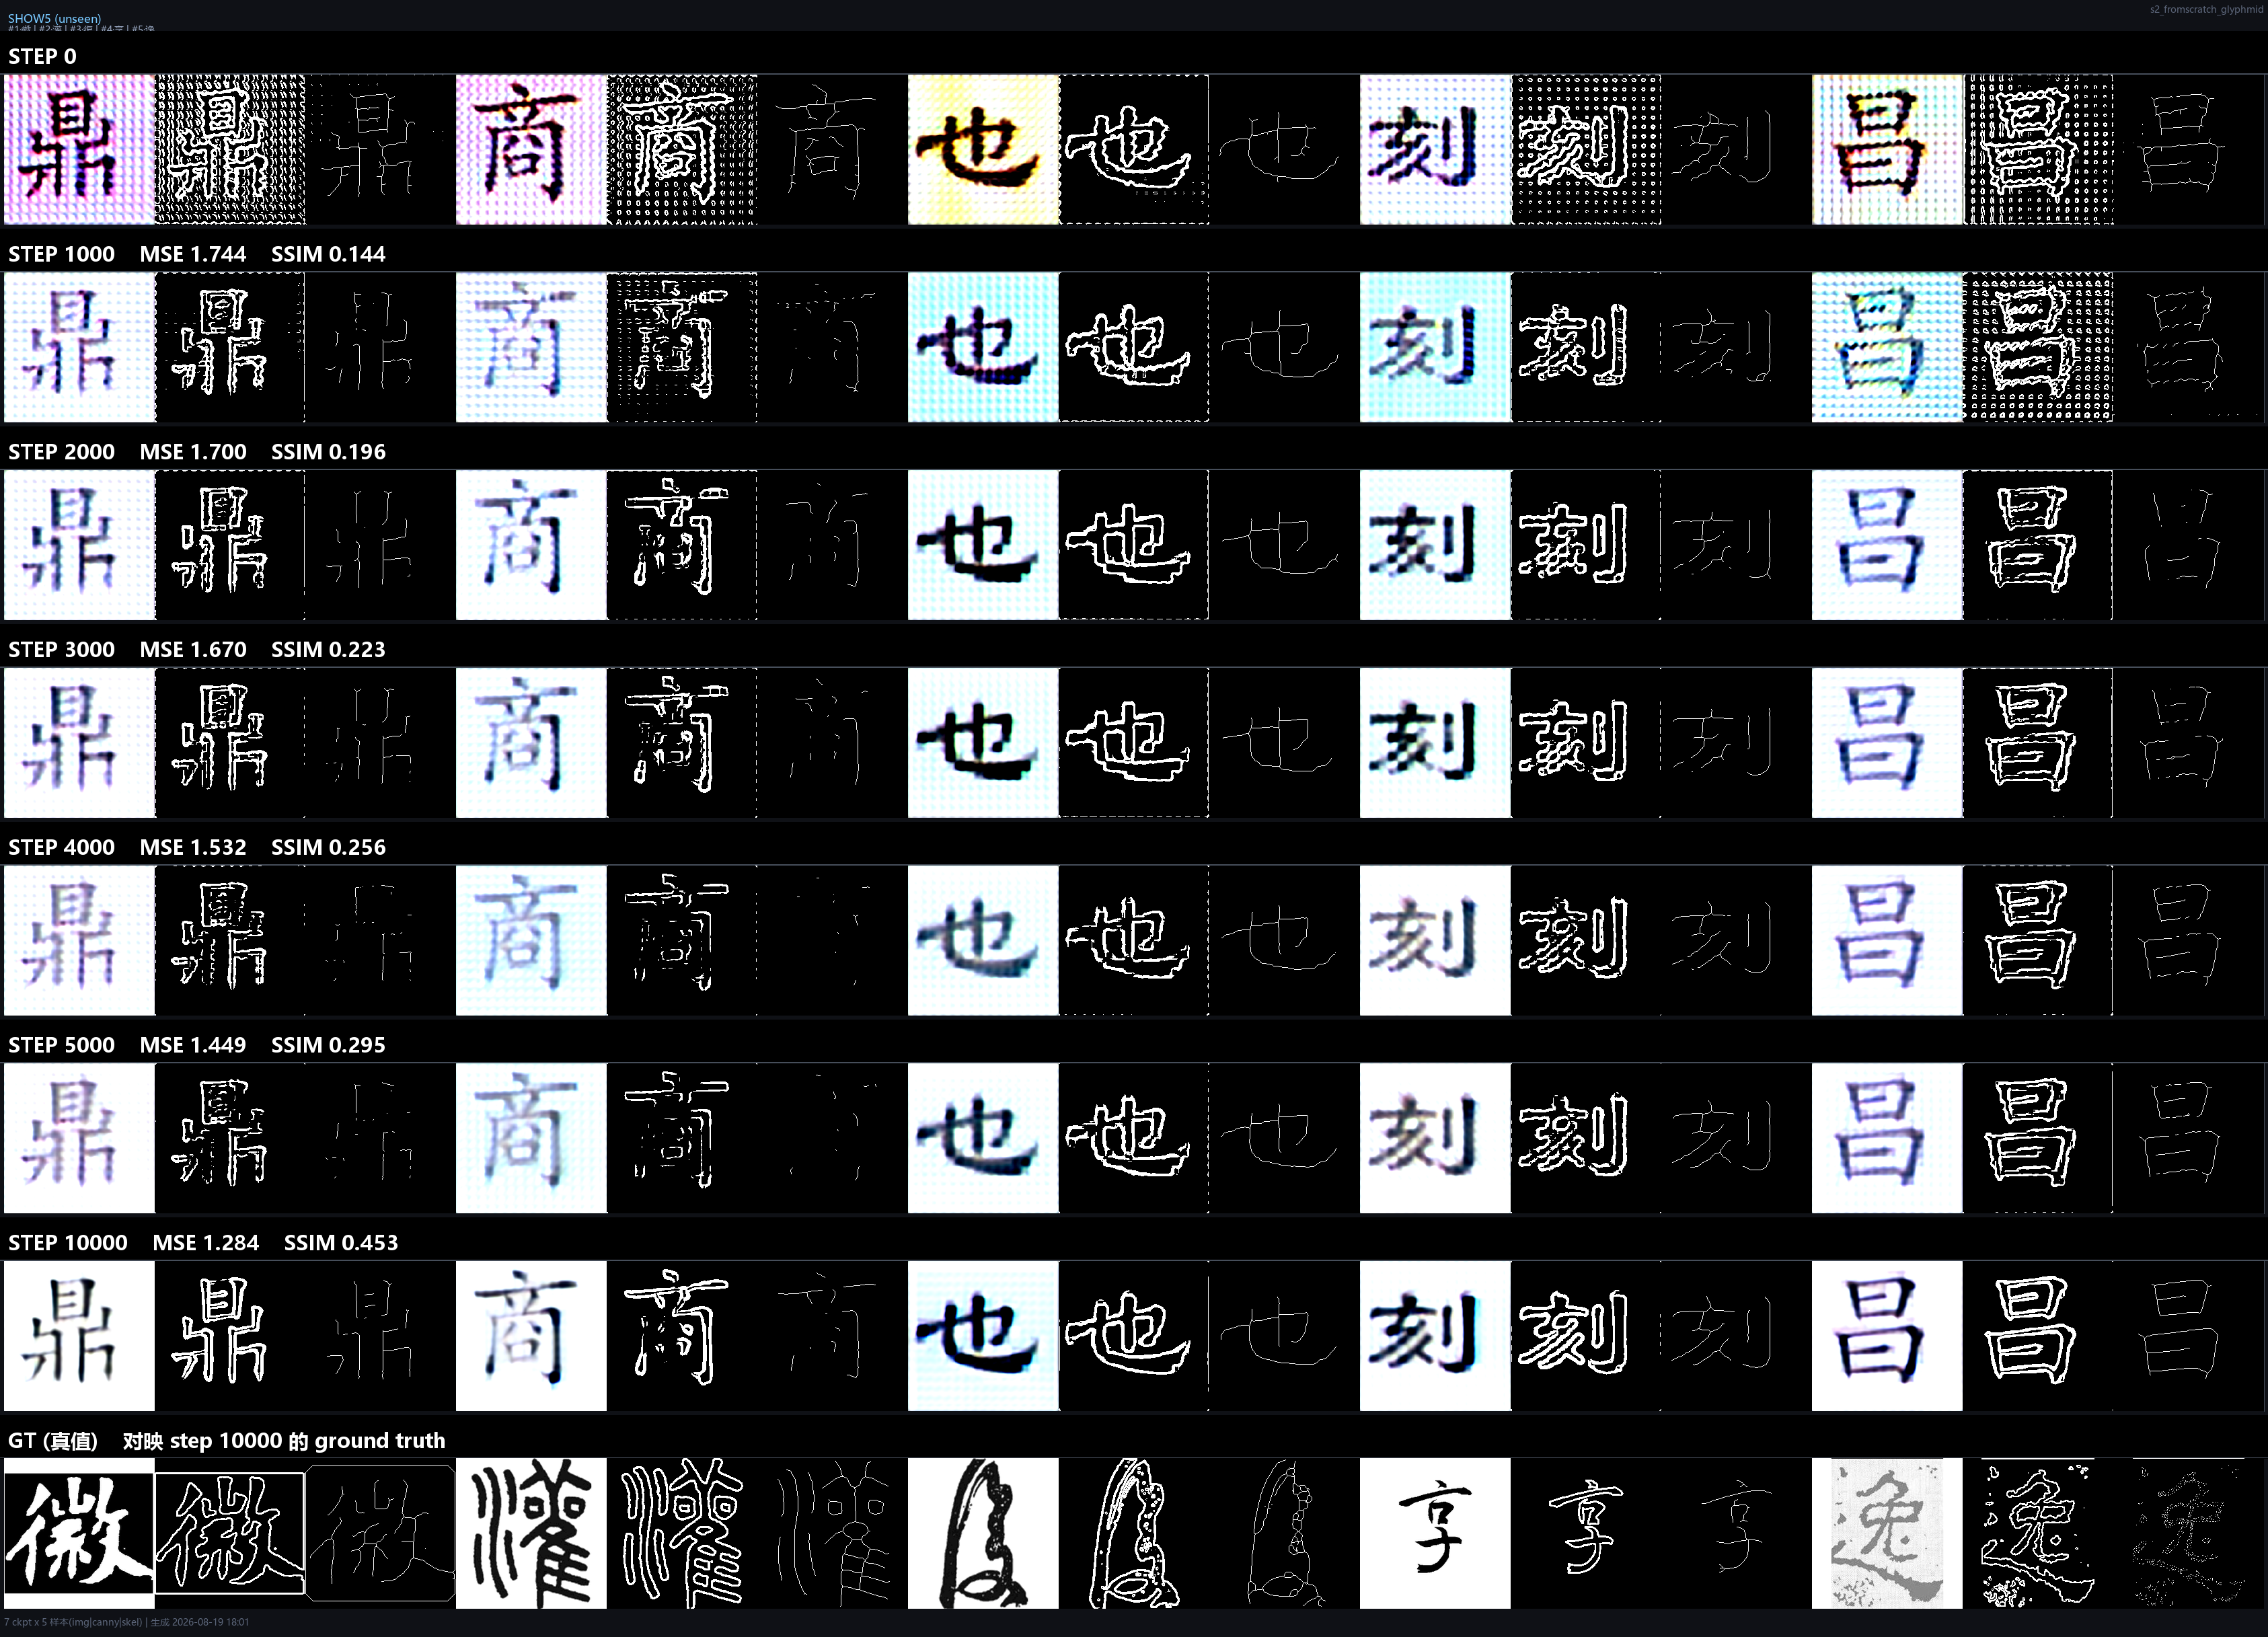
\includegraphics[width=\textwidth,height=0.9\textheight,keepaspectratio]{s2_fromscratch_glyphmid.png}
\caption{s2\_fromscratch\_glyphmid：训练快照（图中按 step 标注 MSE/SSIM）。}
\end{figure}
\clearpage

\subsection{s5\_2factor\_top30（5 书纯两因子主基线，SSIM 0.520）}
\textbf{条件}：S，5 书 top30（128842 行），纯两因子，无字形/结构辅助，大 batch 192，训练上限 200k（当前 eval 至 70k）。\\
\textbf{分析}：多书场景下纯两因子 SSIM 0.520，略低于单书楷书 0.577，符合预期——多书任务对抗/遗忘更强（5 种书体风格差异大）。大 batch 192 有助于稳定训练，但 SSIM 仍有提升空间。作为多书主基线，后续实验应以此为对比基准。

\par\bigskip\clearpage
\begin{figure}[p]
\centering
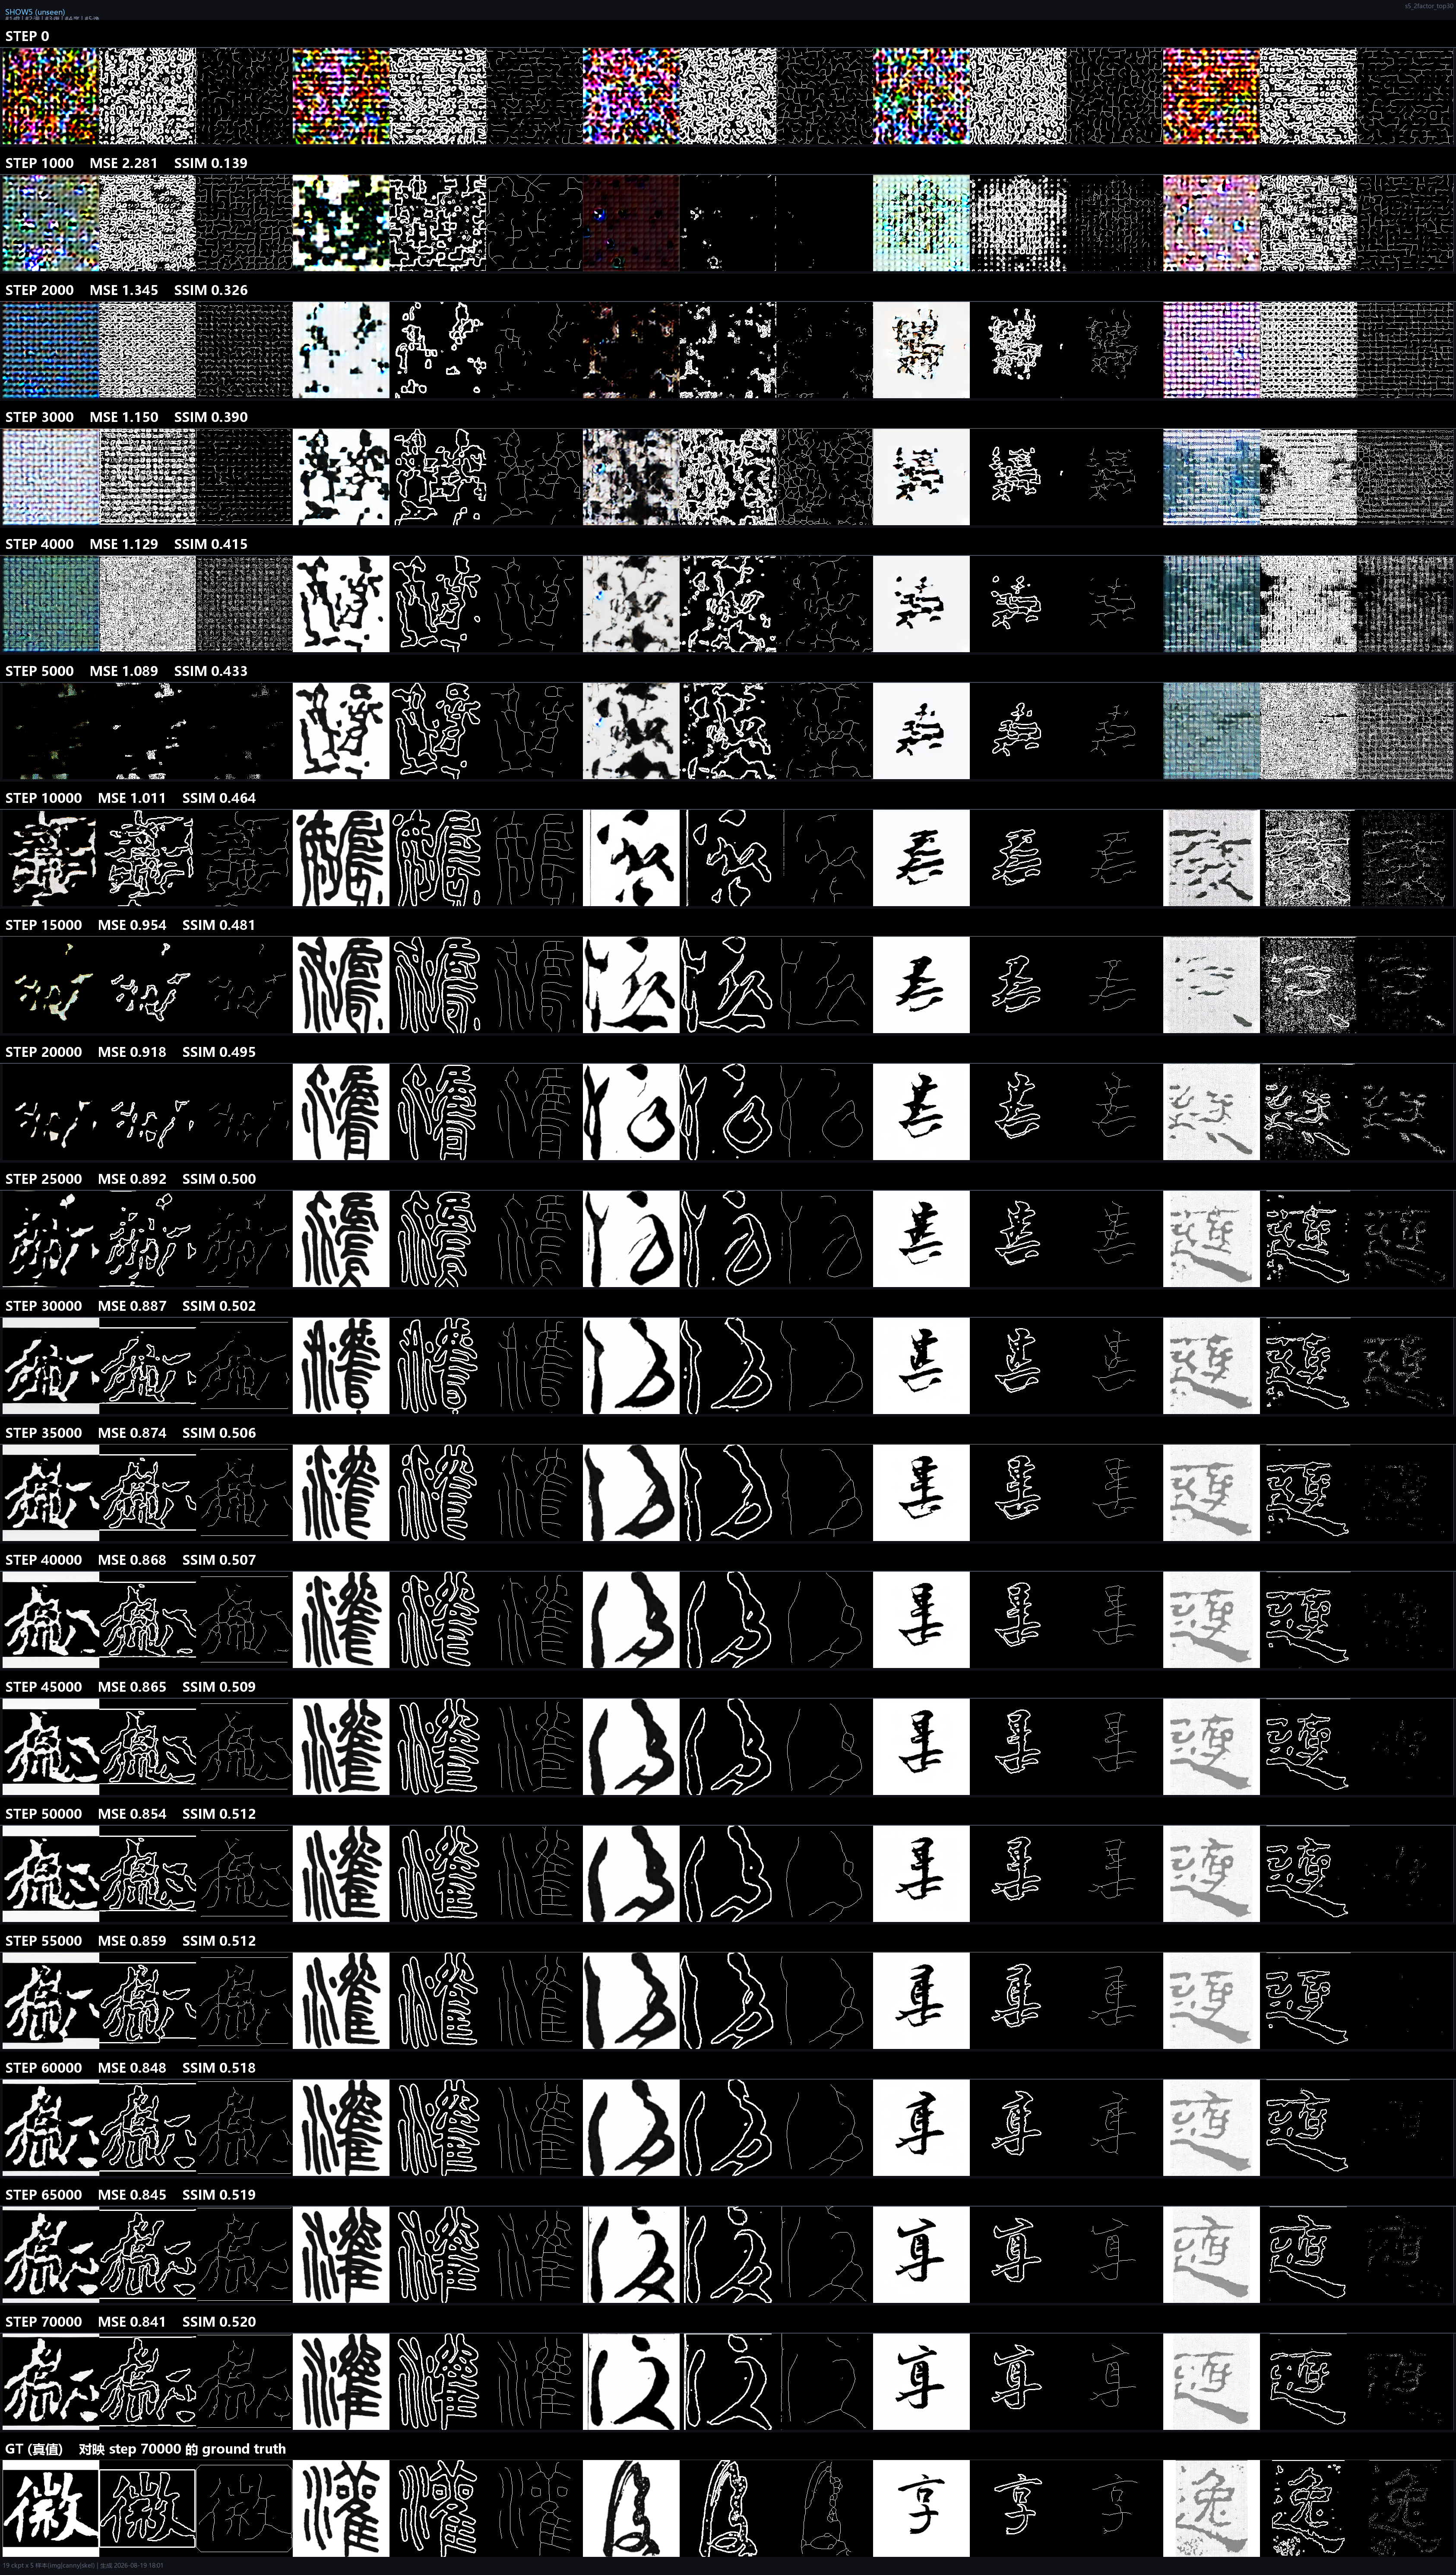
\includegraphics[width=\textwidth,height=0.9\textheight,keepaspectratio]{s5_2factor_top30.png}
\caption{s5\_2factor\_top30：训练快照（图中按 step 标注 MSE/SSIM）。}
\end{figure}
\clearpage

\subsection{s5\_2factor\_struct\_post50k（5 书 + 像素结构损失，SSIM 0.508）}
\textbf{条件}：S，5 书 top30，纯两因子 + 像素域 canny+skel 结构损失（\texttt{w\_canny}=0.5，\texttt{w\_skel}=0.5），50k 后才叠加结构监督，batch 12（内存受限），eval 至 60k。\\
\textbf{分析}：SSIM 0.508 略低于无结构基线 0.520。像素结构损失（canny/skel）旨在提升边缘/骨架形态，但未带来 SSIM 提升，反而略降。可能原因：(1) 结构损失权重（0.5+0.5）与主 MSE 损失冲突；(2) 像素域结构监督在 latent 扩散框架下不够直接（latent 空间与像素空间非线性映射）；(3) 50k 后才叠加结构监督，训练时长不足。小 batch 12 也可能影响收敛。

\par\bigskip\clearpage
\begin{figure}[p]
\centering
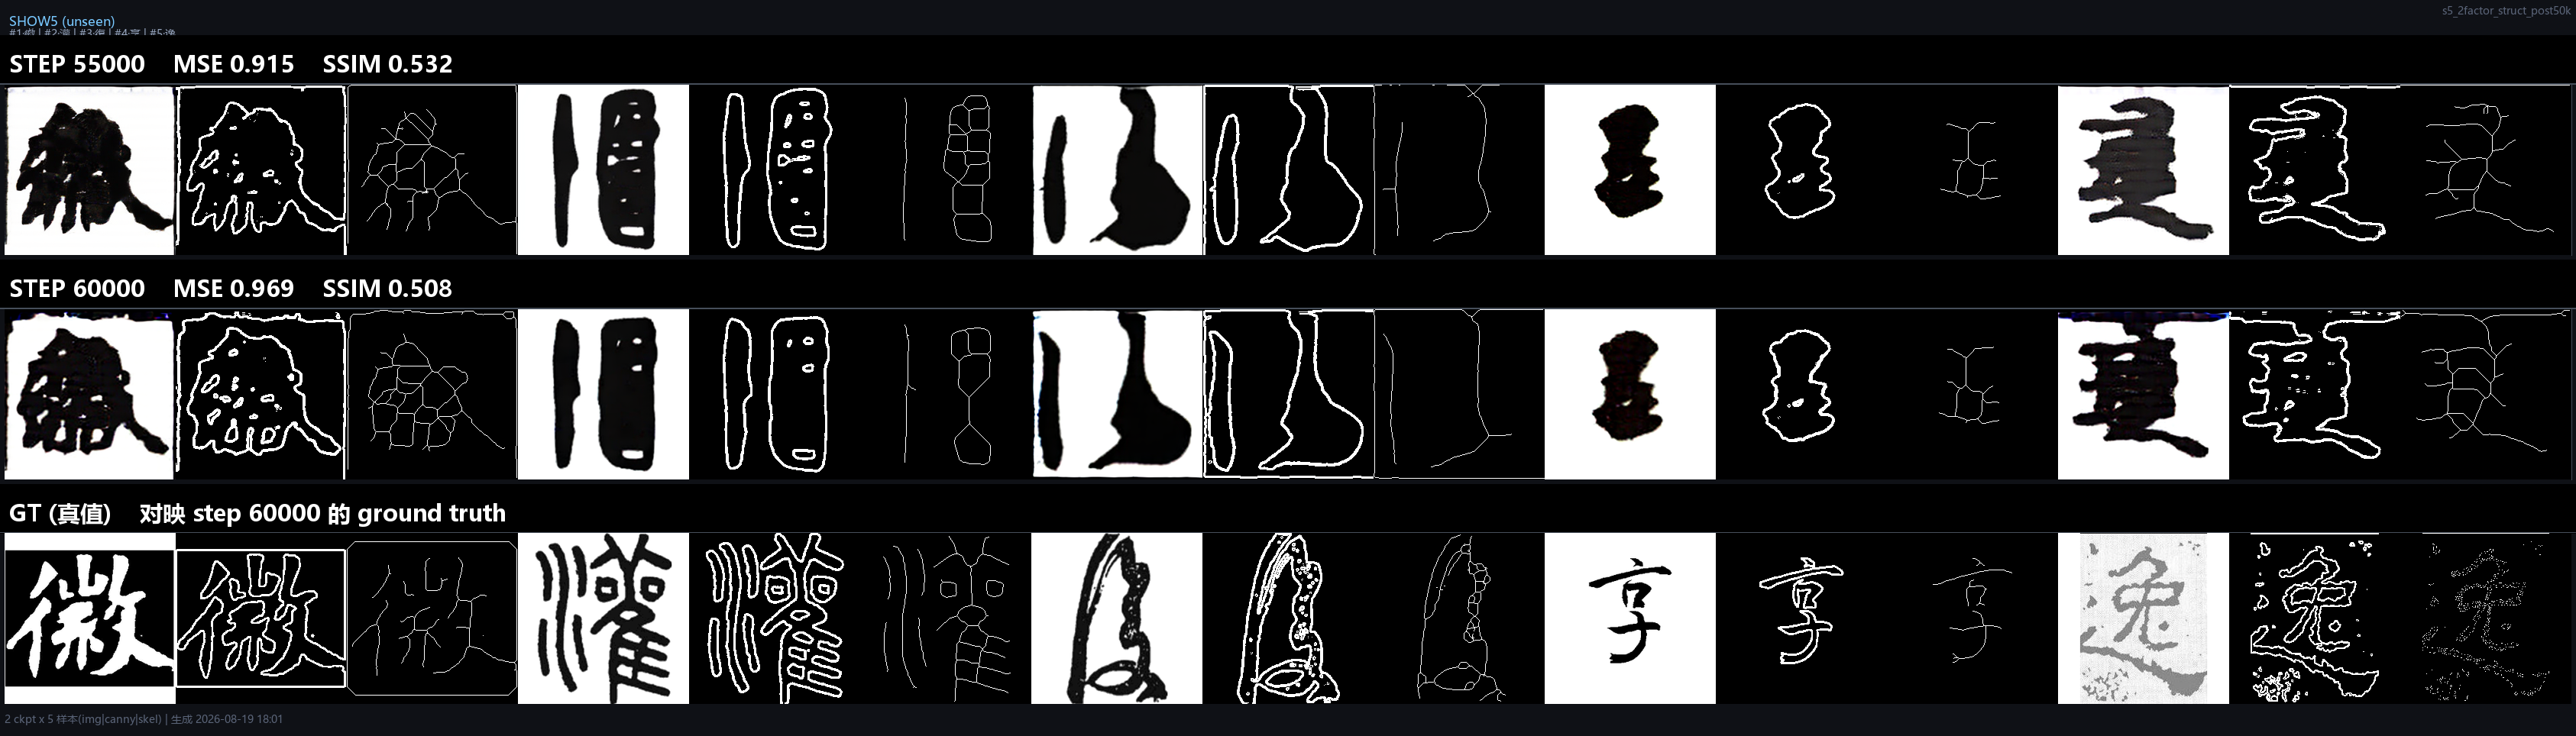
\includegraphics[width=\textwidth,height=0.9\textheight,keepaspectratio]{s5_2factor_struct_post50k.png}
\caption{s5\_2factor\_struct\_post50k：训练快照（图中按 step 标注 MSE/SSIM）。}
\end{figure}
\clearpage

\subsection{s5\_2factor\_B\_latentstruct（B + latent canny 结构，SSIM 0.507）}
\textbf{条件}：DiT-2Cond-B/2（hidden 768），5 书 top30，两因子 + latent 域 canny 结构损失（\texttt{w\_latent\_canny}=0.5，\texttt{latent\_struct\_max\_t}=500），batch 64，eval 至 130k。\\
\textbf{分析}：SSIM 0.507 与 S 多书基线 0.520 接近，略低。B 模型容量更大（hidden 768 vs S 的 2048 维？需确认），但 latent 域 canny 结构损失未带来明显增益。latent 域结构监督理论上更直接（在 latent 空间做 canny），但实际效果与像素域相当。训练至 130k，收敛较深。

\par\bigskip\clearpage
\begin{figure}[p]
\centering
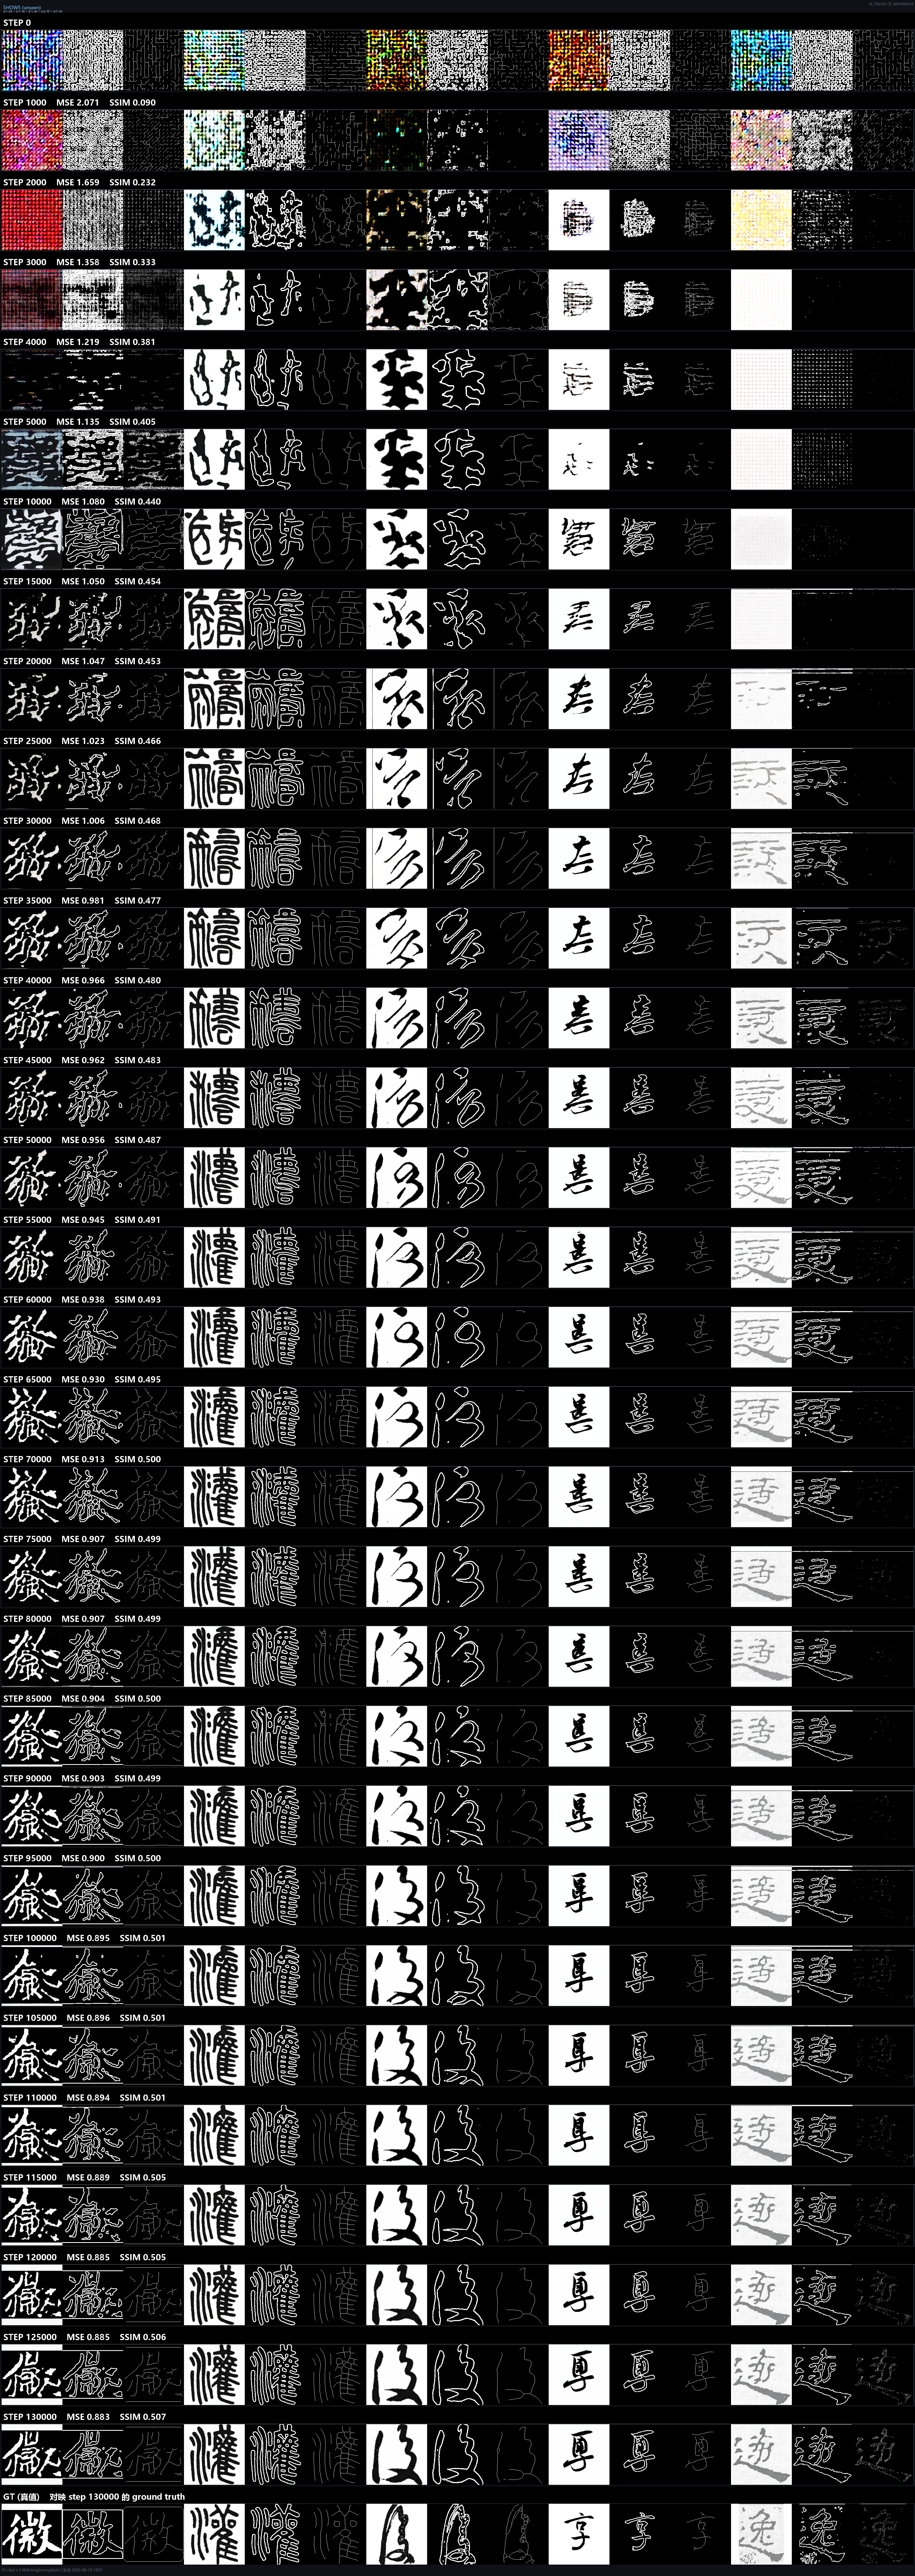
\includegraphics[width=\textwidth,height=0.9\textheight,keepaspectratio]{s5_2factor_B_latentstruct.png}
\caption{s5\_2factor\_B\_latentstruct：训练快照（图中按 step 标注 MSE/SSIM）。}
\end{figure}
\clearpage

\subsection{s5\_2factor\_B\_latentstruct\_pixelsk\_opt（B + 像素 skel，SSIM 0.391）}
\textbf{条件}：B，5 书 top30，两因子 + 像素域 skel（\texttt{w\_skel}=1.0，无 canny），bf16 解码，\texttt{struct\_subset}=16，batch 64，eval 至 115k。\\
\textbf{分析}：SSIM 0.391 显著低于其他 B 变体（0.482--0.507）。仅像素 skel 监督（无 canny）效果最差，可能原因：(1) 骨架监督过于稀疏（细化后仅单像素宽），梯度信号弱；(2) bf16 解码精度不足导致结构损失计算误差；(3) subset=16 解码 batch 过大可能引入数值不稳定。该实验配置不推荐。

\par\bigskip\clearpage
\begin{figure}[p]
\centering
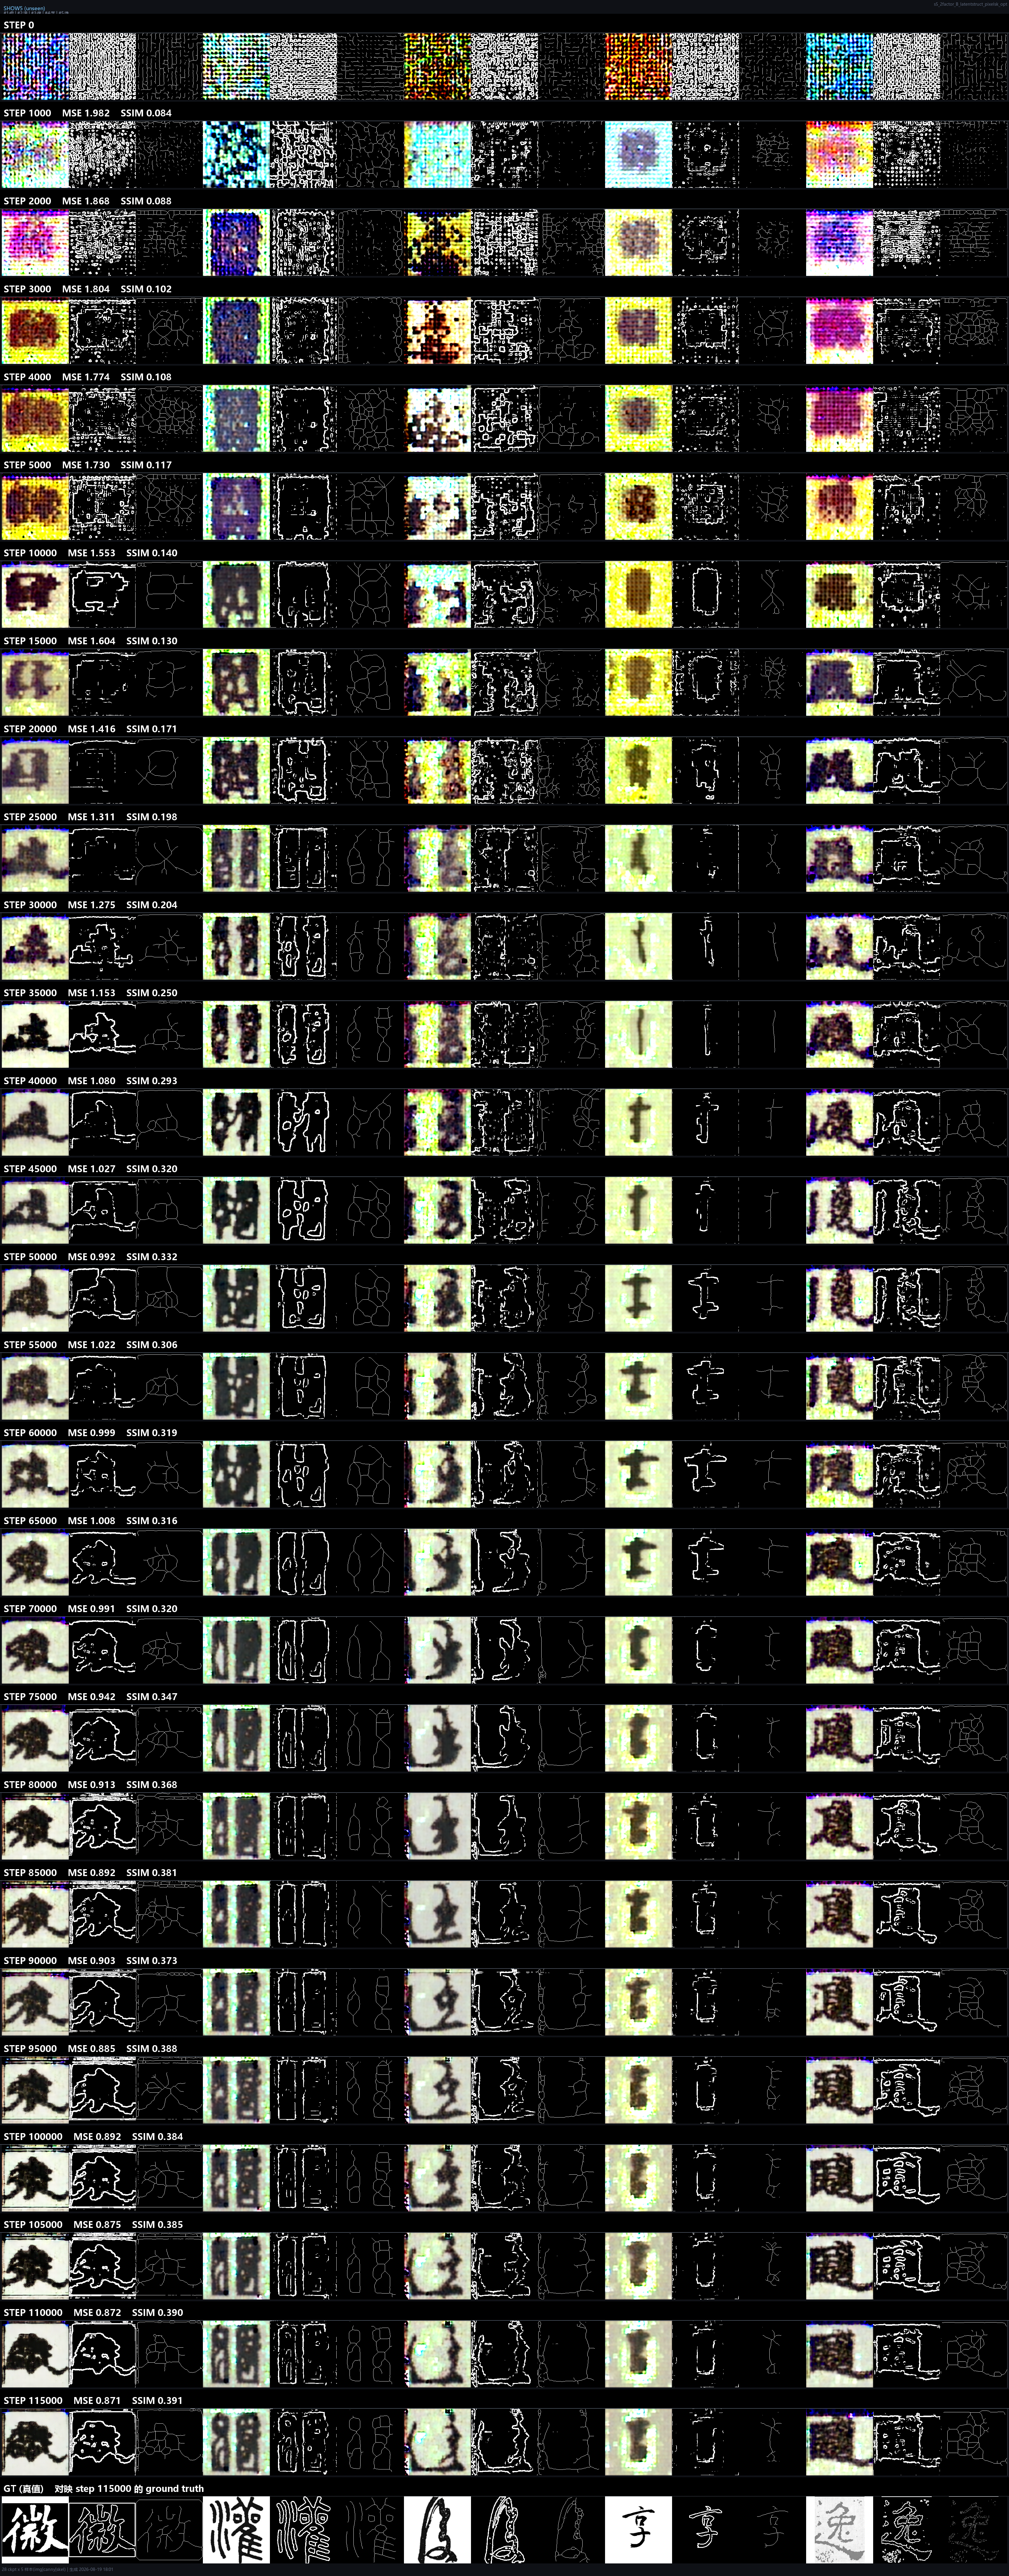
\includegraphics[width=\textwidth,height=0.9\textheight,keepaspectratio]{s5_2factor_B_latentstruct_pixelsk_opt.png}
\caption{s5\_2factor\_B\_latentstruct\_pixelsk\_opt：训练快照（图中按 step 标注 MSE/SSIM）。}
\end{figure}
\clearpage

\subsection{s5\_2factor\_B\_canny05\_pixelsk（B + 像素 canny+skel bf16，SSIM 0.482）}
\textbf{条件}：B，5 书 top30，两因子 + 像素域 canny+skel（\texttt{w\_canny}=0.5，\texttt{w\_skel}=1.0），bf16 解码，\texttt{subset}=16，batch 64，训练较深（eval 至 325k）。\\
\textbf{分析}：SSIM 0.482，B 系列中较高（仅次于 latentstruct 0.507）。完整像素 canny+skel 监督 + bf16 解码 + 长训练（325k）带来较好效果。但 SSIM 仍低于 S 基线 0.520，说明 B 模型容量优势未体现。bf16 解码在此配置下稳定（subset=16 未 OOM），训练收敛。

\par\bigskip\clearpage
\begin{figure}[p]
\centering

\includegraphics[width=\textwidth,height=0.9\textheight,keepaspectratio]{s5_2factor_B_canny05_pixelsk.png}
\caption{s5\_2factor\_B\_canny05\_pixelsk：训练快照（图中按 step 标注 MSE/SSIM）。}
\end{figure}
\clearpage

\subsection{s5\_2factor\_B\_pixelfp32（B + 像素 canny+skel fp32，运行中，SSIM 0.183@35k）}
\textbf{条件}：B，5 书 top30，两因子 + 像素 canny+skel（权重同上），fp32 解码（\texttt{struct\_decode\_bf16=false}，\texttt{subset}=8），batch 32，训练上限 300k，当前已到约 35.5k。\\
\textbf{分析}：SSIM 0.183@35k，相比 20k 的 0.156 仍在缓慢上升、未收敛（与 bf16 同配置 325k 时 0.482 差距仍大）。fp32 解码显存占用大（subset=8 在 24.5G 4090 上安全），训练速度慢。当前指标不能作为 B 与 S 对比依据，需等待收敛。预期随训练深入 SSIM 会继续上升，但能否超越 S 基线 0.520 存疑（参考 bf16 同配置 0.482，而同为 fp32 的收敛上限未知）。

\par\bigskip\clearpage
\begin{figure}[p]
\centering
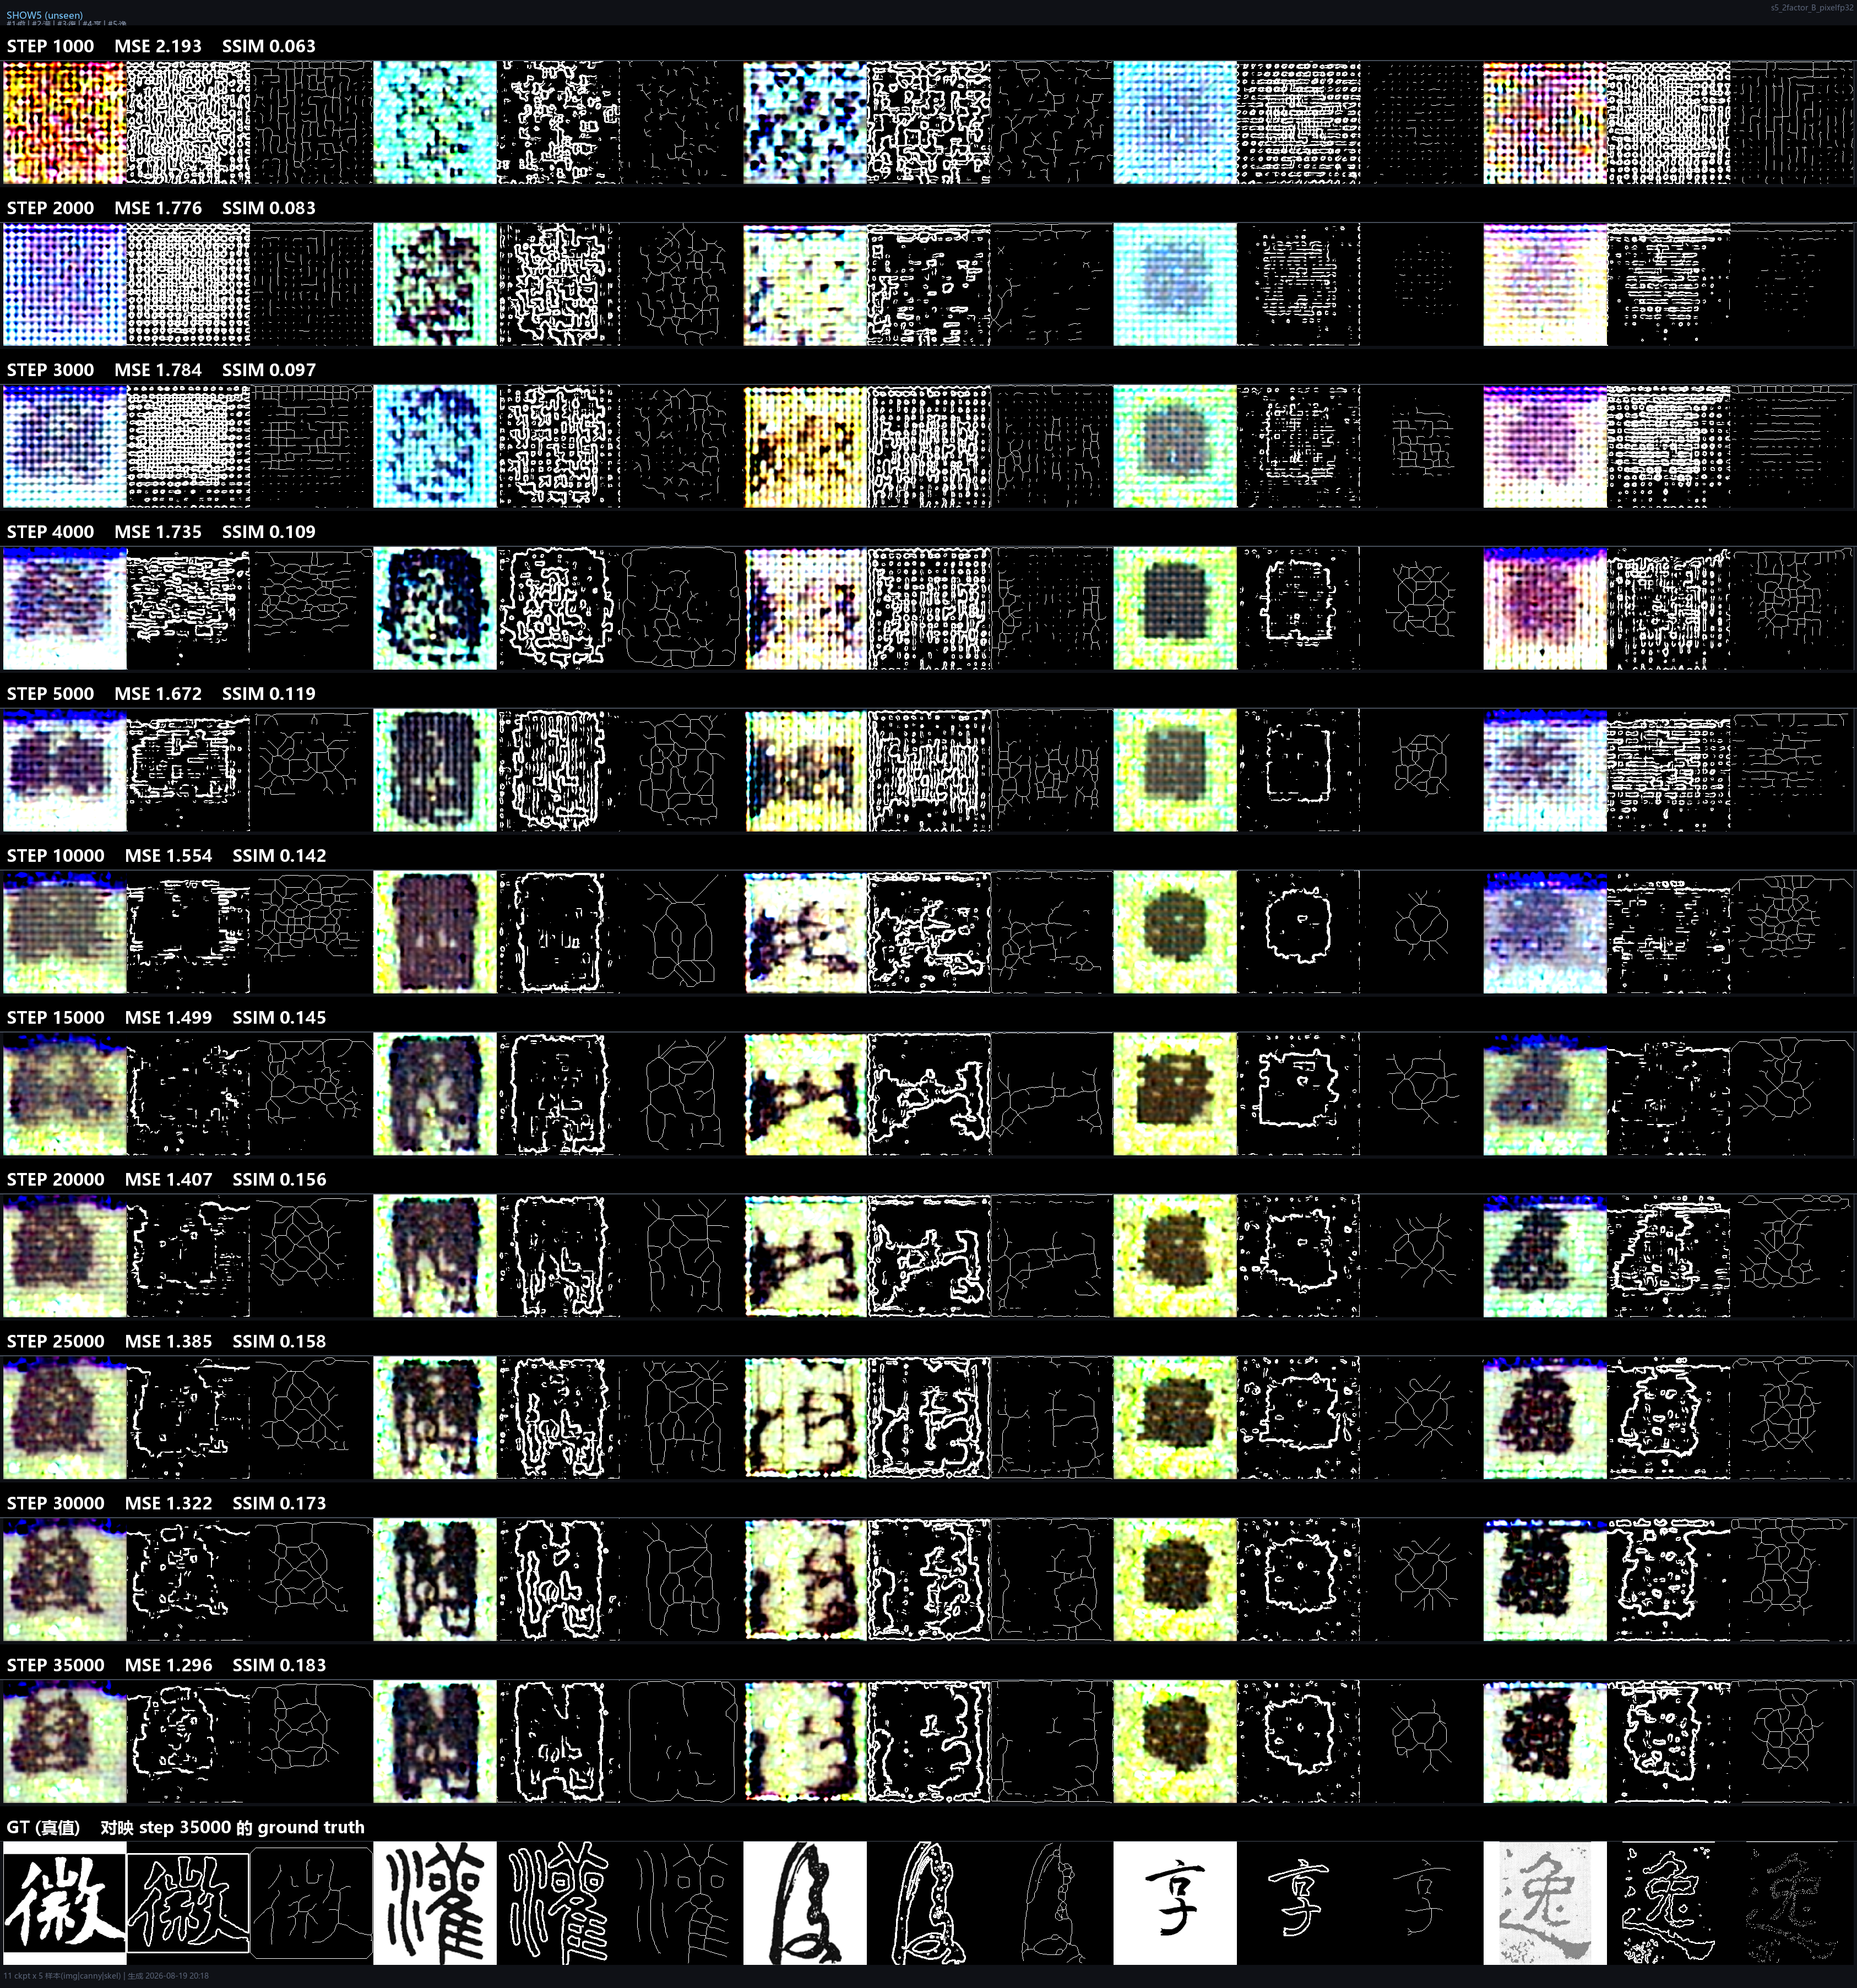
\includegraphics[width=\textwidth,height=0.9\textheight,keepaspectratio]{s5_2factor_B_pixelfp32.png}
\caption{s5\_2factor\_B\_pixelfp32：训练快照（运行中，图中按 step 标注 MSE/SSIM）。}
\end{figure}
\clearpage

\subsection{v3b\_xl\_glyphcond（XL+LoRA + 字形条件，SSIM 0.489）}
\textbf{条件}：DiT-2Cond-XL/2（预训练 DiT-XL-2 + LoRA r=16），楷书单书，两因子 + 标准字形条件（\texttt{w\_glyph\_cond}），融合 \texttt{xl\_highdim}，batch 16，30k。\\
\textbf{分析}：SSIM 0.489，低于 S 单书基线 0.577。XL 预训练 + LoRA 微调 + 字形条件未带来优势，可能原因：(1) XL 模型在书法数据上过参数化（数据量相对小，易过拟合）；(2) 字形条件引入额外复杂度但未提升质量；(3) 训练时长不足（30k vs S 的 50k）。LoRA 微调可能限制了模型适配能力。

\par\bigskip\clearpage
\begin{figure}[p]
\centering
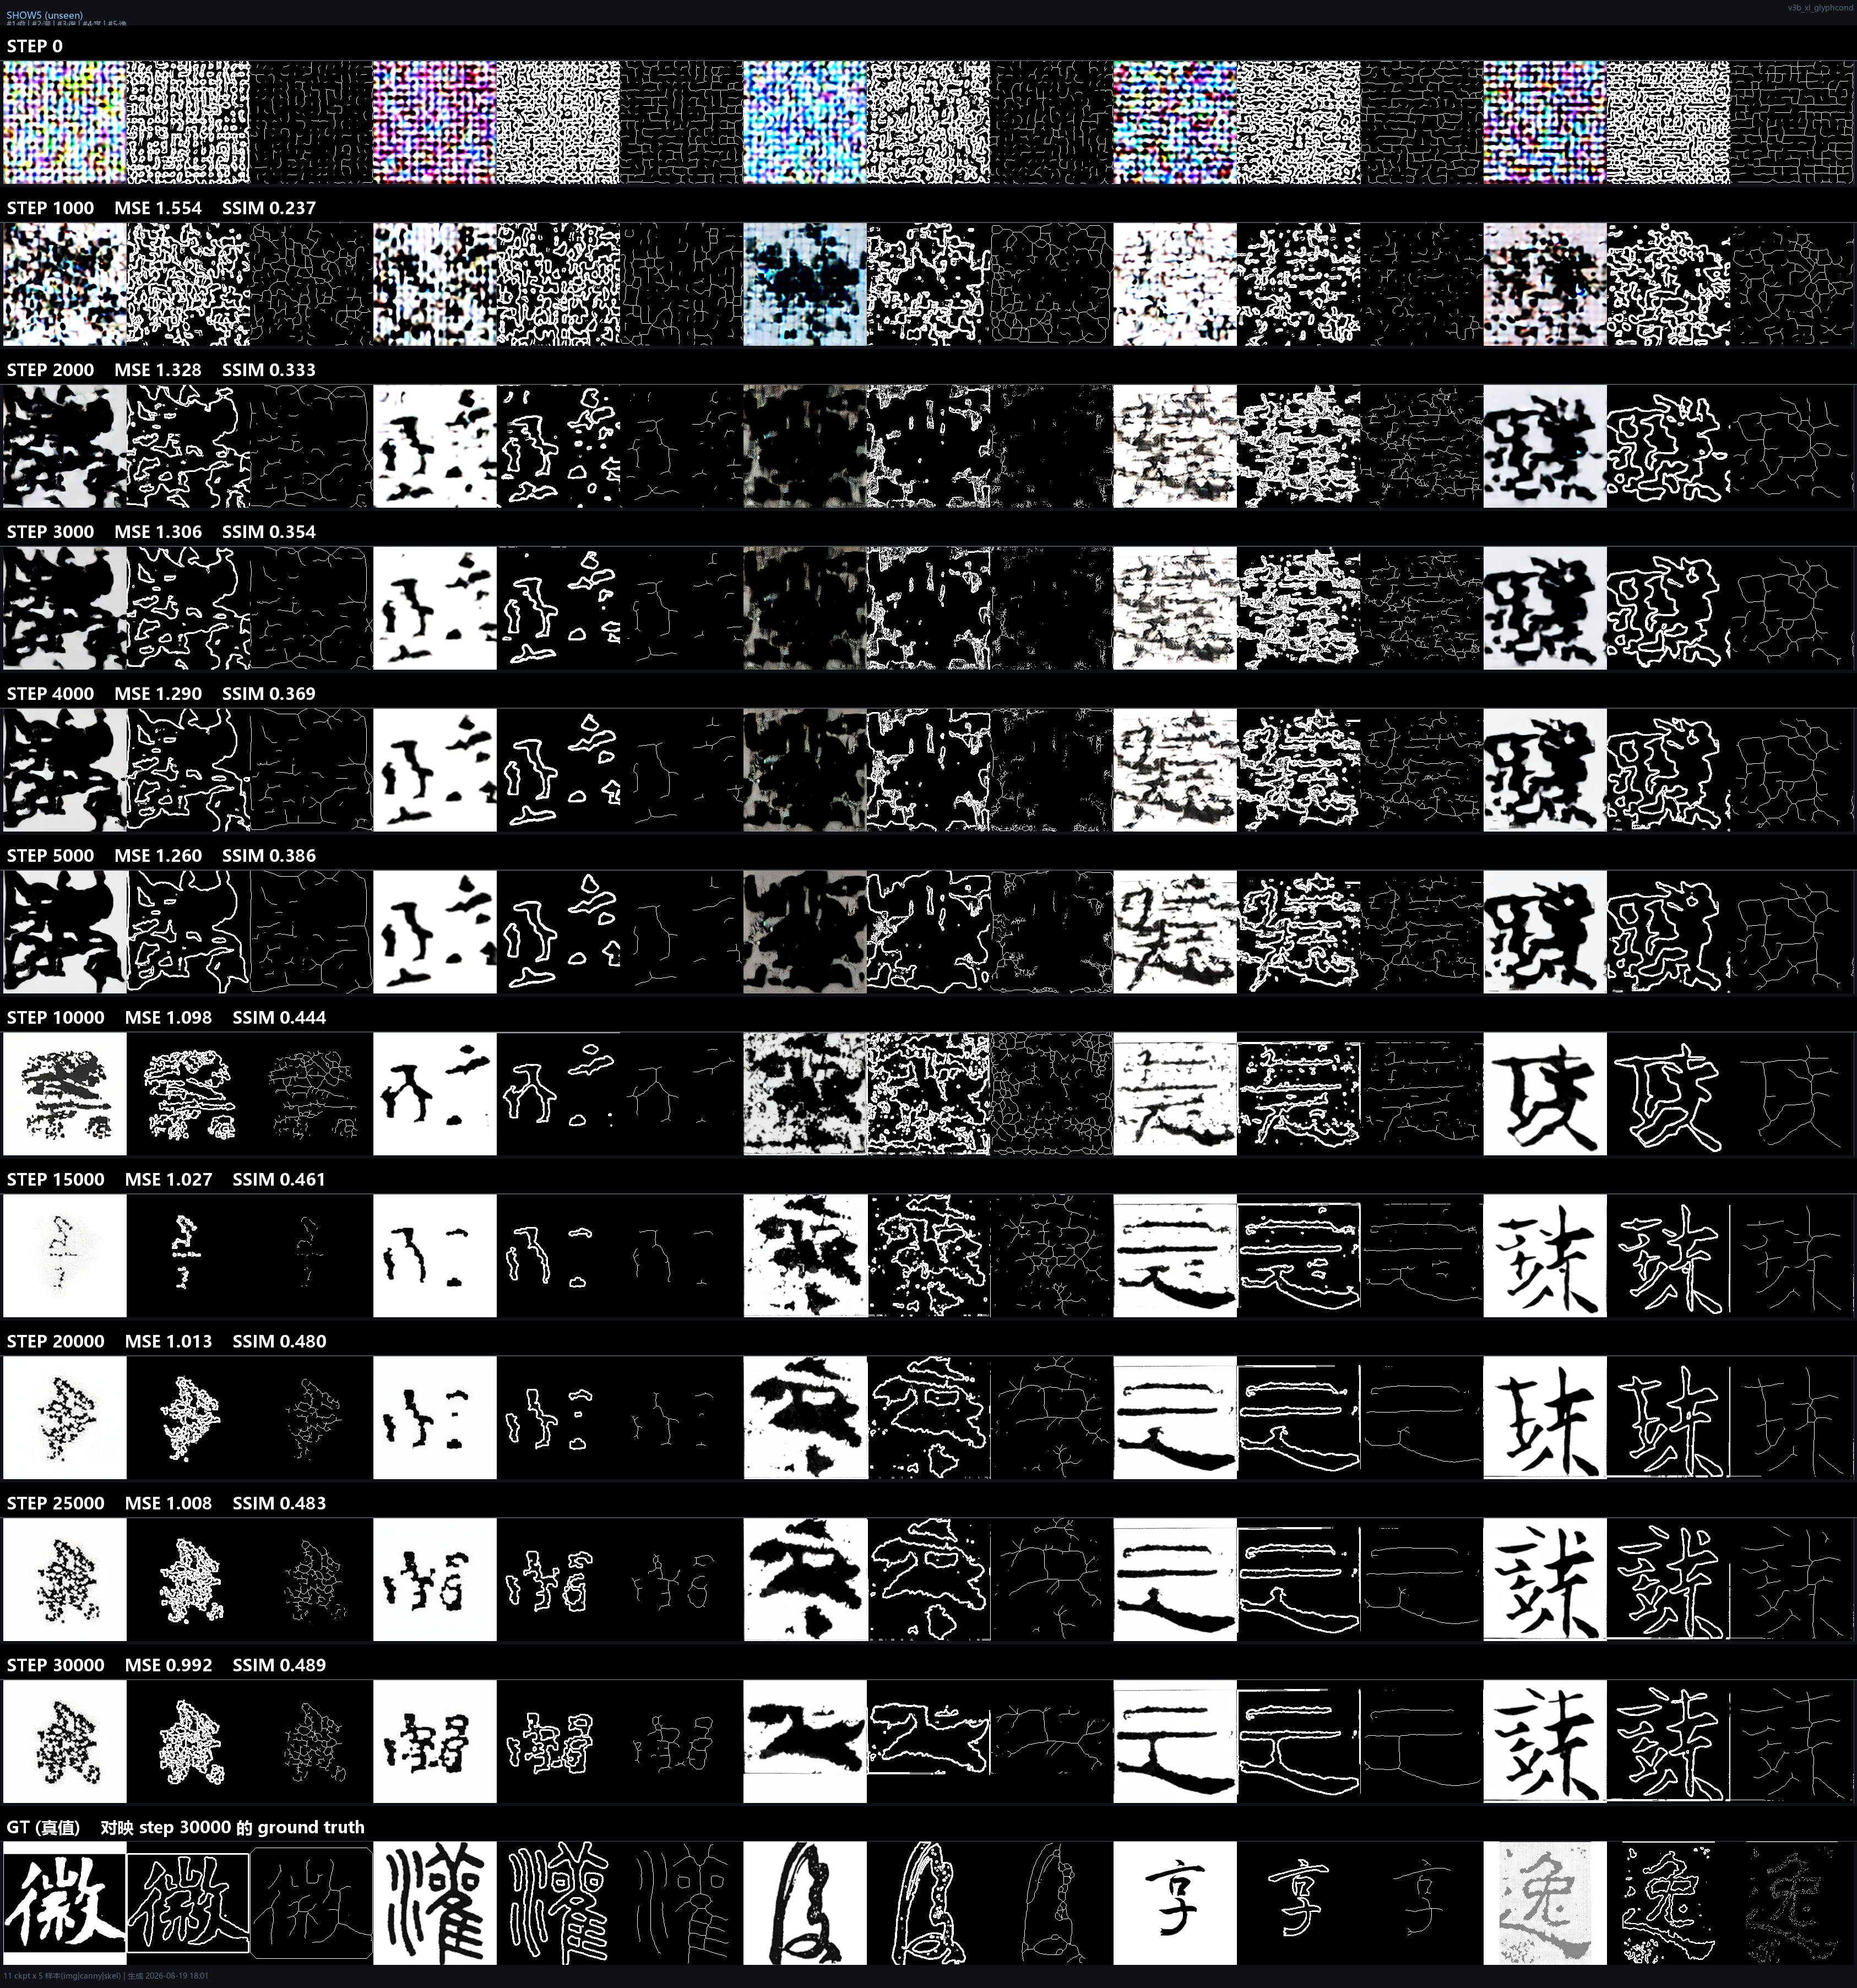
\includegraphics[width=\textwidth,height=0.9\textheight,keepaspectratio]{v3b_xl_glyphcond.png}
\caption{v3b\_xl\_glyphcond：训练快照（图中按 step 标注 MSE/SSIM）。}
\end{figure}
\clearpage

\subsection{v3c\_xl\_glyphcond\_midstep（XL+LoRA + 字形 + 中间步监督，eval 未完成）}
\textbf{条件}：XL+LoRA，楷书单书，同 v3b 但增加标准字形中间步监督（\texttt{w\_std\_mid}=0.8），30k；目前仅保存 1 档 show5 样本，eval100 未跑完，无指标。\\
\textbf{分析}：无指标可分析。参考 s2\_glyphmid（字形中间步监督 SSIM 0.453 低于基线 0.577），预期 v3c 也不会优于 v3b（0.489）。中间步字形监督在多个实验中均未带来正增益。

\par\bigskip\clearpage
\begin{figure}[p]
\centering
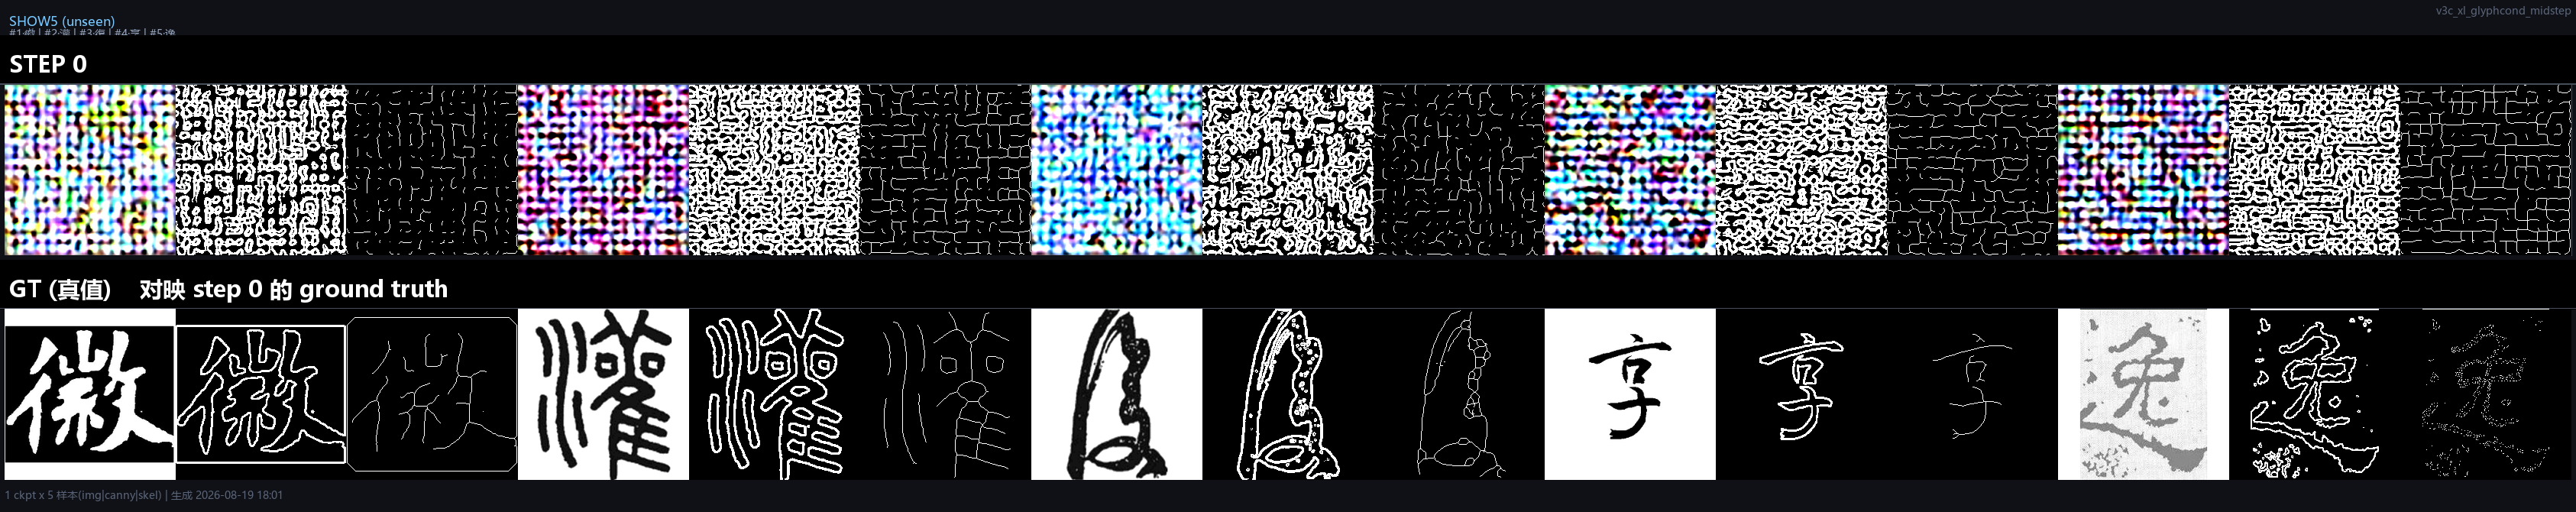
\includegraphics[width=\textwidth,height=0.9\textheight,keepaspectratio]{v3c_xl_glyphcond_midstep.png}
\caption{v3c\_xl\_glyphcond\_midstep：训练快照（运行中/未完成 eval）。}
\end{figure}
\clearpage

\section{Insight 与结论}

\subsection{S 模型优于 B 模型}
纯两因子下，小模型 S（楷书 SSIM 0.577、5 书 0.520）显著高于 5 书 B 各变体（0.507 / 0.482 / 0.391）。
B 模型容量更大（hidden 768 vs S 的 2048 维？需确认实际参数量），但在给定数据/结构监督下，更大容量并未换来更好的重建/匹配质量。
B 系列继续投入训练的性价比存疑——即使 fp32 变体收敛，参考 bf16 同配置 0.482，也难以超越 S 基线 0.520。
\textbf{建议}：后续实验优先在 S 尺度上探索，B/XL 仅在特殊场景（如超高分辨率、超长序列）考虑。

\subsection{标准字形/中间步监督未提升 SSIM}
s2\_glyphmid（0.453）低于纯两因子 s2（0.577），v3b（0.489）含字形条件而 XL 也未见优势。
字形中间步监督对评价指标带来的是负效应，可能原因：
\begin{itemize}
  \item 中间步监督权重过大（0.8）导致梯度冲突，干扰主任务学习；
  \item 标准字形（渲染字体）与训练数据（真实书法）分布不匹配，监督信号有偏；
  \item 训练时长不足，中间步监督需要更长训练才能见效。
\end{itemize}
\textbf{建议}：若继续使用字形监督，降低权重（如 0.2--0.4）或延迟到训练后期叠加；或改用真实书法字形（而非渲染字体）作为监督目标。

\subsection{结构损失改善观感但不提升 SSIM}
canny/skel 系列（0.391--0.508）整体不高于无结构基线，结构监督更多影响边缘/骨架形态，未反映在 SSIM 上，甚至常使其略降。
可能原因：
\begin{itemize}
  \item 像素域结构监督在 latent 扩散框架下不够直接（latent 空间与像素空间非线性映射）；
  \item 结构损失权重与主 MSE 损失冲突，需更精细的权重调度；
  \item SSIM 指标本身对边缘/骨架敏感度不足，结构损失可能在视觉上提升但 SSIM 未体现。
\end{itemize}
\textbf{建议}：结构损失可作为辅助监督保留（改善视觉质量），但不应作为主要优化目标；或改用更敏感的指标（如 LPIPS、FID）评估结构质量。

\subsection{多书 vs 单书}
5 书 S 纯两因子（0.520）低于单书楷书 S（0.577），多书任务的对抗/遗忘可能更强。
5 种书体风格差异大（楷书端正、篆书圆润、草书连绵、行书流畅、隶书扁平），模型需同时拟合多种分布，难度更高。
\textbf{建议}：多书场景可考虑书体条件显式建模（如书体 embedding + 书体-书家交互），或分书体训练独立模型。

\subsection{fp32 朴素解码尚未收敛}
B\_pixelfp32（20k 时 SSIM 0.156 $\to$ 35k 时 0.183）与 bf16 同配置（B\_canny05 325k 时 0.482）差距仍大，需更久训练才能下结论。
fp32 解码显存占用大（subset=8 在 24.5G 4090 上安全），训练速度慢（约 1.4 step/s）。
\textbf{建议}：继续训练至收敛（预期 100k--200k），若最终 SSIM 仍在 0.4--0.5 区间，则与 bf16 无本质差异，fp32 解码无必要。

\subsection{总体建议}
\begin{itemize}
  \item \textbf{优先 S 模型}：在给定数据规模下，S 模型性价比最高，B/XL 未带来明显增益。
  \item \textbf{纯两因子已足够}：无需字形条件、中间步监督、结构损失，纯两因子 callig$\times$char 已达最佳 SSIM。
  \item \textbf{多书场景需进一步探索}：当前多书 SSIM 0.520 仍有提升空间，可尝试书体显式建模或分书体训练。
  \item \textbf{停止低效实验}：B 系列、XL 系列、字形/中间步监督、结构损失均未带来正增益，建议停止投入，聚焦 S 模型多书优化。
\end{itemize}

\end{document}
